\chapter{Optical potentials}

\textit{In the introduction we emphasized the importance of optical lattices,
yet we left out many details, for instance, how these optical lattices are
created and how the optical quantities enter the potential energy of the
atoms. In this chapter we will make up for said gaps. First we will
recapitulate the theory behind laser light intensities and then derive a
formulation of the effective lattice potentials felt by the atoms.}

\section{Atom-light interaction}

At first we need to ask ourselves how the laser field acts as a perturbation
to the Hamiltonian of the atomic system and how this perturbation leads to an
intensity dependent potential for the atoms, which we can control in the
experiment. In deviations are loosely based on
references~\cite{Gerry2004,Jackson2005,Bartelmann2018}.

\subsection{Dipole potential}

We will use \gls{si} units unless stated otherwise. The Hamiltonian of an electron
in an external electromagnetic field reads
\begin{equation}
  \hat{H}_\text{em}
  =\frac{1}{2m_e}{\left(\hat{\vb{p}}+e\vb{A}\right)}^2-e\Phi+\hat{V}_0
  \label{eq:hamiltonian_em},
\end{equation}
with vector potential $\vb{A}$ and scalar potential $\Phi$ of the external
field and the Coulomb potential of the nucleus $\hat{V}_0$. Further $m_e$
denotes the electron mass and $e$ the elementary charge.
\Cref{eq:hamiltonian_em} is exact for the hydrogen atom that only hosts one
electron. For alkali atoms we know that inner electron shells are closed and
the single outer electron is approximately described by
\cref{eq:hamiltonian_em}. The electromagnetic field relates to the
vector and scalar potential through
\begin{align}
  \vb{E}=-\grad{\Phi}-\pdv{\vb{A}}{t}, &&
  \vb{B}=\curl{\vb{A}},
  \label{eq:field_em_potentials}
\end{align}
where $\vb{E}$ is the electric and $\vb{B}$ the magnetic field component.

The canonical momentum $\hat{\vb{p}}+e\vb{A}$ in \cref{eq:hamiltonian_em} is
difficult to work with. Fortunately Gauge transforms
\begin{align}
  \vb{A}\to\vb{A}+\grad{\chi}
  &&
  \Phi\to\Phi-\pdv{\chi}{t}
  \label{eq:gauge_transform_em}
\end{align}
allow us to simplify \cref{eq:hamiltonian_em} by choosing a specific Gauge
function $\chi(\vb{x},t)$. The Gauge function itself $\chi$ does not amend the
electromagnetic field components \cref{eq:field_em_potentials} which we
usually consider to represent physical reality --- in contrast to the
electromagnetic potentials $\vb{A},\Phi$ which are usually only considered
mathematical aid.\footnote{The Aharonov-Bohm effect actually provides evidence
that aso the electromagnetic potentials represent physical reality.} In the
following we choose the gauge function $\chi=-\vb{A}\cdot\vb{x}$ and assume
the dipole approximation $\vb{A}(\vb{x},t)\approx\vb{A}(t)$. The dipole
approximation neglects the spatial variation of the electromagnetic field
over the atom and instead assumes a small separation of opposite charges at
the nucleus. The dipole approximation is reasonable as wave length of visible
light are much larger than atomic length scales~\cite{Gerry2004}. In the dipole
approximation $\chi$ satisfies the Coulomb gauge condition
$\divergence{\vb{A}}=0$ allowing us to set $\Phi=0$ as no external sources are
present~\cite{Jackson2005}. Finally we can rewrite
\cref{eq:hamiltonian_em} as
\begin{equation}
  \hat{H}_\text{dip}
  =\frac{\hat{\vb{p}}^2}{2m}+\hat{V}_0+\hat{V}_\text{dip}
  =\hat{H}_0+\hat{V}_\text{dip}
  \label{eq:hamiltonian_dip}
\end{equation}
with the dipole potential
\begin{equation}
  \hat{V}_\text{dip}
  =-\hat{\vb{d}}\cdot\vb{E}
  \label{eq:potential_dip},
\end{equation}
the dipole operator $\hat{\vb{d}}=-e\vb{x}$ and the spatially homogeneous
light field $\vb{E}(t)$.

\subsection{AC-Stark effect}

We are now going to solve \cref{eq:hamiltonian_dip} for an arbitrary light
field of the form
\begin{equation}
  \vb{E}(t,\vb{x})
  =\vb{E}_0(\vb{x})\cos(\omega t)
  \label{eq:light_field}
\end{equation}
where $\vb{E}_0(\vb{x})$ should be compatible with Maxwell's equations and
be approximately constant on atomic length scales to not violate the dipole
approximation. Further we need the laser frequency $\omega$ to be
far-off-resonant to the atomic transition frequencies to avoid population
dynamics.

At $t<0$ the system is in the energy eigenstate $\ket{n}$ of the
unperturbated Hamiltonian $\hat{H}_0$
\begin{equation}
  \hat{H}_0\ket{n}
  =E_n\ket{n}
  =\hbar\omega_n\ket{n}
  \label{eq:eigenvalue_energy_unperturbated}.
\end{equation}
At $t>0$ the external light field appears immediately. The new state
$\ket{\psi}$ can be expanded in the complete basis of the previous energy
eigenstates
\begin{equation}
  \ket{\psi}
  =
  \sum_n{c_n(t)}{e^{-i{\omega_n}t}}\ket{n}
  \label{eq:state_expansion_unperturbated}.
\end{equation}
Inserting \cref{eq:state_expansion_unperturbated} into the time-dependent
Schrödinger equation with the dipole Hamiltonian \cref{eq:hamiltonian_dip} and
applying $\bra{m}{e^{i{\omega_m}t}}$ to the right hand side leads us to a set
of differential equations
\begin{equation}
  \dot{c}_m
  =
  -\frac{i}{\hbar}\sum_n{c_n(t)}{e^{-i\omega_{nm}t}}
  \bra{m}\hat{V}_\text{dip}\ket{n}
  \label{eq:differential_equation_population_dynamics}
\end{equation}
with $\omega_{nm}=\omega_n-\omega_m$. One can read
\cref{eq:differential_equation_population_dynamics} as the rate by which
the probability amplitude of a state $m$ changes in time. It is equal to the
sum of oscillations between states $n$ and $m$ weighted by the current
probability of state $c_n(t)$ and the interaction strength. If we are able to
solve \cref{eq:differential_equation_population_dynamics} for $c_n(t)$ the
population dynamic is entirely described by the time-dependent probabilities
$\abs{c_n(t)}^2$. By using \cref{eq:light_field} we can rewrite the dipole
transition matrix elements
\begin{equation}
  \bra{m}\hat{V}_\text{dip}\ket{n}
  =\Omega_{nm}(\vb{x})\cos(\omega t)\hbar
  \label{eq:elements_dipole_transition_matrix}
\end{equation}
where we introduced the Rabi frequency
\begin{equation}
  \Omega_{nm}(\vb{x})
  =\bra{n}\hat{\vb{d}}\cdot\vb{E}_0(\vb{x})\ket{m}/\hbar
  \label{eq:rabi_frequency}.
\end{equation}
More general expressions for dipole transition elements of one and two
electron systems can be found in Reference~\cite{Bethe1957}. 

\subsubsection{Two-level system}

From now on we assume a two state system that initially is in the ground
state $c_g(0)=1,c_e(0)=0$. Under these circumstances the dynamics described in
\cref{eq:differential_equation_population_dynamics} simplify to
\begin{align}
  i\dot{c}_g=\Omega_{ge}c_e(t)\cos(\omega t)e^{+i\omega_0 t} &&
  i\dot{c}_e=\Omega_{ge}c_g(t)\cos(\omega t)e^{-i\omega_0 t}
  \label{eq:differential_equation_population_dynamics_two_state_system}
\end{align}
Writing $\cos(\omega t)$ in terms of exponential functions and dropping
$e^{\pm i(\omega+\omega_{ge})t}$ yields the so-called \gls{rwa}
\begin{align}
  i\dot{c}_g\approx\frac{\Omega_{ge}}{2}c_e(t)e^{+i\Delta\omega t} &&
  i\dot{c}_e\approx\frac{\Omega_{ge}}{2}c_g(t)e^{-i\Delta\omega t}
  \label{eq:differential_equation_population_dynamics_two_state_system_rwa}
\end{align}
where we introduced the frequency detuning
$\Delta\omega=\abs{\omega-\omega_0}$. The \gls{rwa} is motivated by the fact
that oscillations of frequency $\omega+\omega_0$ are fast compared to changes
in the population dynamics and therefore vanish on average.

We now define $a_g=c_g$ and $a_e=c_e e^{i\Delta\omega t}$ and rewrite
\cref{eq:differential_equation_population_dynamics_two_state_system_rwa} by
\begin{align}
  i\dot{a}_g=\frac{\Omega_{ge}}{2}a_e(t) &&
  i\dot{a}_e=\frac{\Omega_{ge}}{2}a_g(t)-a_e\Delta\omega
  \label{eq:differential_equation_population_dynamics_two_state_system_shift}.
\end{align}
Using
\cref{eq:differential_equation_population_dynamics_two_state_system_shift} we
can diagonalize the Hamiltonian and find the energy eigenvalues to be
\begin{equation}
  E_{e,g}
  =\frac{\hbar}{2}\left(-\Delta\omega\mp\sqrt{\Omega_{ge}^2+\Delta\omega^2}\right)
  \approx
  \mp\frac{\hbar\Omega_{ge}^2}{4\Delta\omega}
  \label{eq:eigenvalues_energy_light_shift}
\end{equation}
where we applied a Taylor expansion for $\Omega_{ge}/\Delta\omega\ll1$ around
$\Omega_{ge}/\Delta\omega=0$ and omitted terms of higher order.

Consequently, atoms in an external off-resonant light field experience an
effective periodic dipole potential
\begin{equation}
  \hat{V}_\text{eff}(\vb{x})
  =
  \mp\frac{\hbar\Omega_{ge}^2(\vb{x})}{4\Delta\omega}
  =
  \mp\frac{d_0^2E_0^2(\vb{x})}{4\hbar\Delta\omega}
  \label{eq:potential_effective}
\end{equation}
with dipole element $d_0$. The sign has to be chosen with respect to the
direction of the laser detuning from resonance. If the laser is red-shifted
compared to the resonance frequency, $\omega-\omega_0>0$, we need to choose
the negative sign as the particles are drawn towards the areas of maximum
intensity. If the laser is blue-shifted compared to the resonance frequency,
$\omega-\omega_0<0$, we need to choose the positive sign as the particles are
drawn towards the area of minimum intensity. The same results can also be
obtained by the use of second order perturbation theory~\cite{Grimm2008}.

\section{Laser light fields}

In this section our focus will be on the spatial distribution of the lattice
and perturbation laser light fields that create the time-averaged dynamical
potentials we discussed in the introduction.

\subsection{Gaussian beams}

The predominant output mode of most lasers is the fundamental transverse
gaussian mode. For a laser beam propagating along the $z$-direction it is
described by
\begin{equation}
  \vb{E}(r,z)
  =
  \vb{E}_0\frac{w(0)}{w(z)}
  \exp{-\frac{r^2}{w{(z)}^2}}
  \exp{-ik\left(z+\frac{r^2}{2R(z)}-\arctan(\frac{z}{z_R})\right)}
  \label{eq:gaussian_beam}
\end{equation}
where $w{(z)}$ is the waist radius, $z_R=\pi w{(0)}^2/\lambda$ the Rayleigh
range and $R(z)$ the radius of curvature of the beam's wavefront at position
$z$.
\begin{figure}[ht]
  \centering
  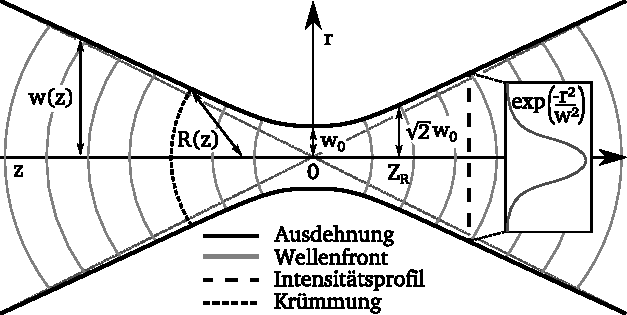
\includegraphics[width=.9\textwidth]{\mediadir{image/gaussian-beam.pdf}}
  \captionsetup{width=.9\textwidth}
  \caption{Illustration of Gaussian beam parameters from Ref.~\cite{Aleph2014}
    translated into English with changed radius of curvature.
  }\label{fig:gaussian_beam}
\end{figure}
\Cref{fig:gaussian_beam} unveils how the parameters relate to the beam
profile as a function of propagation distance $z$. The waist radius $w(z)$
corresponds to the \gls{fwhm} by $w(z)=FWHM(z)/\sqrt{2\ln2}$, $R(z)$ relates
to the wavefront curvature and $z_R$ is the distance from origin $z=0$ where
the beam waist is $w(z)=\sqrt{2}w(0)$. Beam waist and curvature of radius
evolve according to
\begin{align}
  w{(z)}
  =
  w{(0)}{\left[1+{\left(\frac{z}{z_R}\right)}^2\right]}^{1/2}
  &&
  R{(z)}=z{\left[1+{\left(\frac{z_R}{z}\right)}^2\right]}
  \label{eq:gaussian_beam_evolvement}.
\end{align}

Fortunately \cref{eq:potential_effective} only depends on the absolute
square of the electric field, thus we can drop the complex exponential from
\cref{eq:gaussian_beam} to find an expression for the Gaussian intensity
distribution
\begin{equation}
  I(r,z)
  =
  I_0
  {\left(\frac{w(0)}{w(z)}\right)}^2
  \exp{-\frac{2r^2}{w{(z)}^2}}
  =
  I_0
  \frac{\exp{-\frac{2r^2}{w{(z)}^2}}}{1+{\left(\frac{z}{z_R}\right)}^2}
  \label{eq:gaussian_intensity}
\end{equation}
where $I_0$ is the maximum intensity at $r=z=0$.

\subsubsection{Lattice intensity}

A \gls{1d} optical lattices can be generated through the interference
of two counter-propagating Gaussian beams. One way to achieve
counter-propagation while keeping the coherence stable, is to use a mirror.
Under the assumption of perfect reflection of the mirror, the electrical field
component of the laser beam is described by
\begin{align*}
  \vb{E}_\rightarrow(\vb{x},t)+\vb{E}_\leftarrow(\vb{x},t)
  &=
  \vb{E}_0(r,z)\cos(\omega t-kz)+\vb{E}_0(r,z)\cos(\omega t+kz)\\
  &=
  2\vb{E}_0(r,z)\cos(kz)\cos(\omega t).
\end{align*}
Hence, the intensity distribution equals
\cref{eq:gaussian_intensity} with an additional $4\cos^2(kz)$ factor
\begin{equation}
  I(r,z)
  =
  4I_0\cos^2(kz)
  \frac{\exp{-\frac{2r^2}{w{(z)}^2}}}{1+{\left(\frac{z}{z_R}\right)}^2}
  \label{eq:lattice_intensity}
\end{equation}
caused by the constructive interference.
\begin{table}[ht]
  \centering
  \begin{tabular}{cccc}
    \toprule
    Laser wavelength $\lambda$ &
    Lattice constant $a=\lambda/2$ &
    Beam waist $w(0)$ &
    Rayleigh length $z_R$ \\
    \midrule
    \SI{1064}{\nano\meter} &
    \SI{532}{\nano\meter} &
    \SI{150}{\micro\meter} &
    \SI{66}{\milli\meter} \\
    \bottomrule
  \end{tabular}
  \captionsetup{width=.8\textwidth}
  \caption{Typical values for a Gaussian beam used to generate an optical
    lattice potential.
  }\label{tab:gaussian_beam_lattice}
\end{table}
\Cref{tab:gaussian_beam_lattice} lists typical values for a Gaussian beam
used to construct an optical lattice potential. Typical atom clouds occupy
about 50--100 lattice sites spanning over a range of
$l=50a\approx\SI{27}{\micro\meter}$~\cite{Rom2009}. As typical atom clouds
are much smaller then the typical beam waists used for optical lattices, we
have $r/w(z)\ll1$ and can approximate \cref{eq:lattice_intensity}
\begin{equation}
  I(r,z)
  \approx
  4I_0\cos^2(kz)
  \label{eq:gaussian_intensity_approx}
\end{equation}
which we will use from now on as the intensity distribution for \gls{1d}
optical lattices.

\subsubsection{Perturbation intensity}

For the generation of optical lattices we want large beam waists because
otherwise the potential is not homogeneous and there is a potential energy
difference between neighboring lattice sites. For our perturbation potential,
however, we need very high resolution on the order of a single lattice site,
and therefore need a tightly focused beam.
\begin{table}[ht]
  \centering
  \begin{tabular}{cccc}
    \toprule
    Laser wavelength $\lambda$ &
    Beam waist $w(0)$ &
    Rayleigh length $z_R$ \\
    \midrule
    \SI{532}{\nano\meter} &
    \SI{1}{\micro\meter} &
    \SI{6}{\micro\meter} \\
    \bottomrule
  \end{tabular}
  \captionsetup{width=.8\textwidth}
  \caption{Typical values for a Gaussian beam used to perturbate the optical
    lattice potential reported by~\cite{Hertlein2017}.
  }\label{tab:gaussian_beam_perturbation}
\end{table}
\Cref{tab:gaussian_beam_perturbation} summarizes the beam parameter of the
perturbation potential as suggested in Ref.~\cite{Hertlein2017}. For these
parameters approximations made for optical lattice are not valid because of
the small beam waist and Rayleigh length and we need to the exact
\cref{eq:gaussian_intensity} formula. In fact for an actual experiment we
would like to focus the laser beam to even smaller waists. The ultimate goal
would be the ability to address single lattice sites.

\section{Effective local potentials}

With \cref{eq:potential_effective} we found an expression of the potential
energy in terms of atomic properties like the dipole transition element, the
atomic resonance and the laser intensity distribution. For the laser intensity
distribution of the optical lattice we derived
\cref{eq:gaussian_intensity_approx} and we concluded that the intensity of the
laser used for the creation of local potentials obeys
\cref{eq:gaussian_intensity}. If we add these pieces together we can calculate
the effective potential with local perturbation as seen by the atoms. We will
find that its shape deviates from the idealized local potentials we presented
in the introduction in \Cref{fig:optical_lattice_local_pot} and 
\Cref{fig:optical_lattice_local_barrier}.

\subsubsection{Barrier}

One embodiment of local potentials we described in the introduction was the
barrier potential. A barrier potential confines atoms to a subspace of the
global lattice and could be used to model thermodynamical equilibrium
processes.
\begin{figure}[ht]
  \centering
  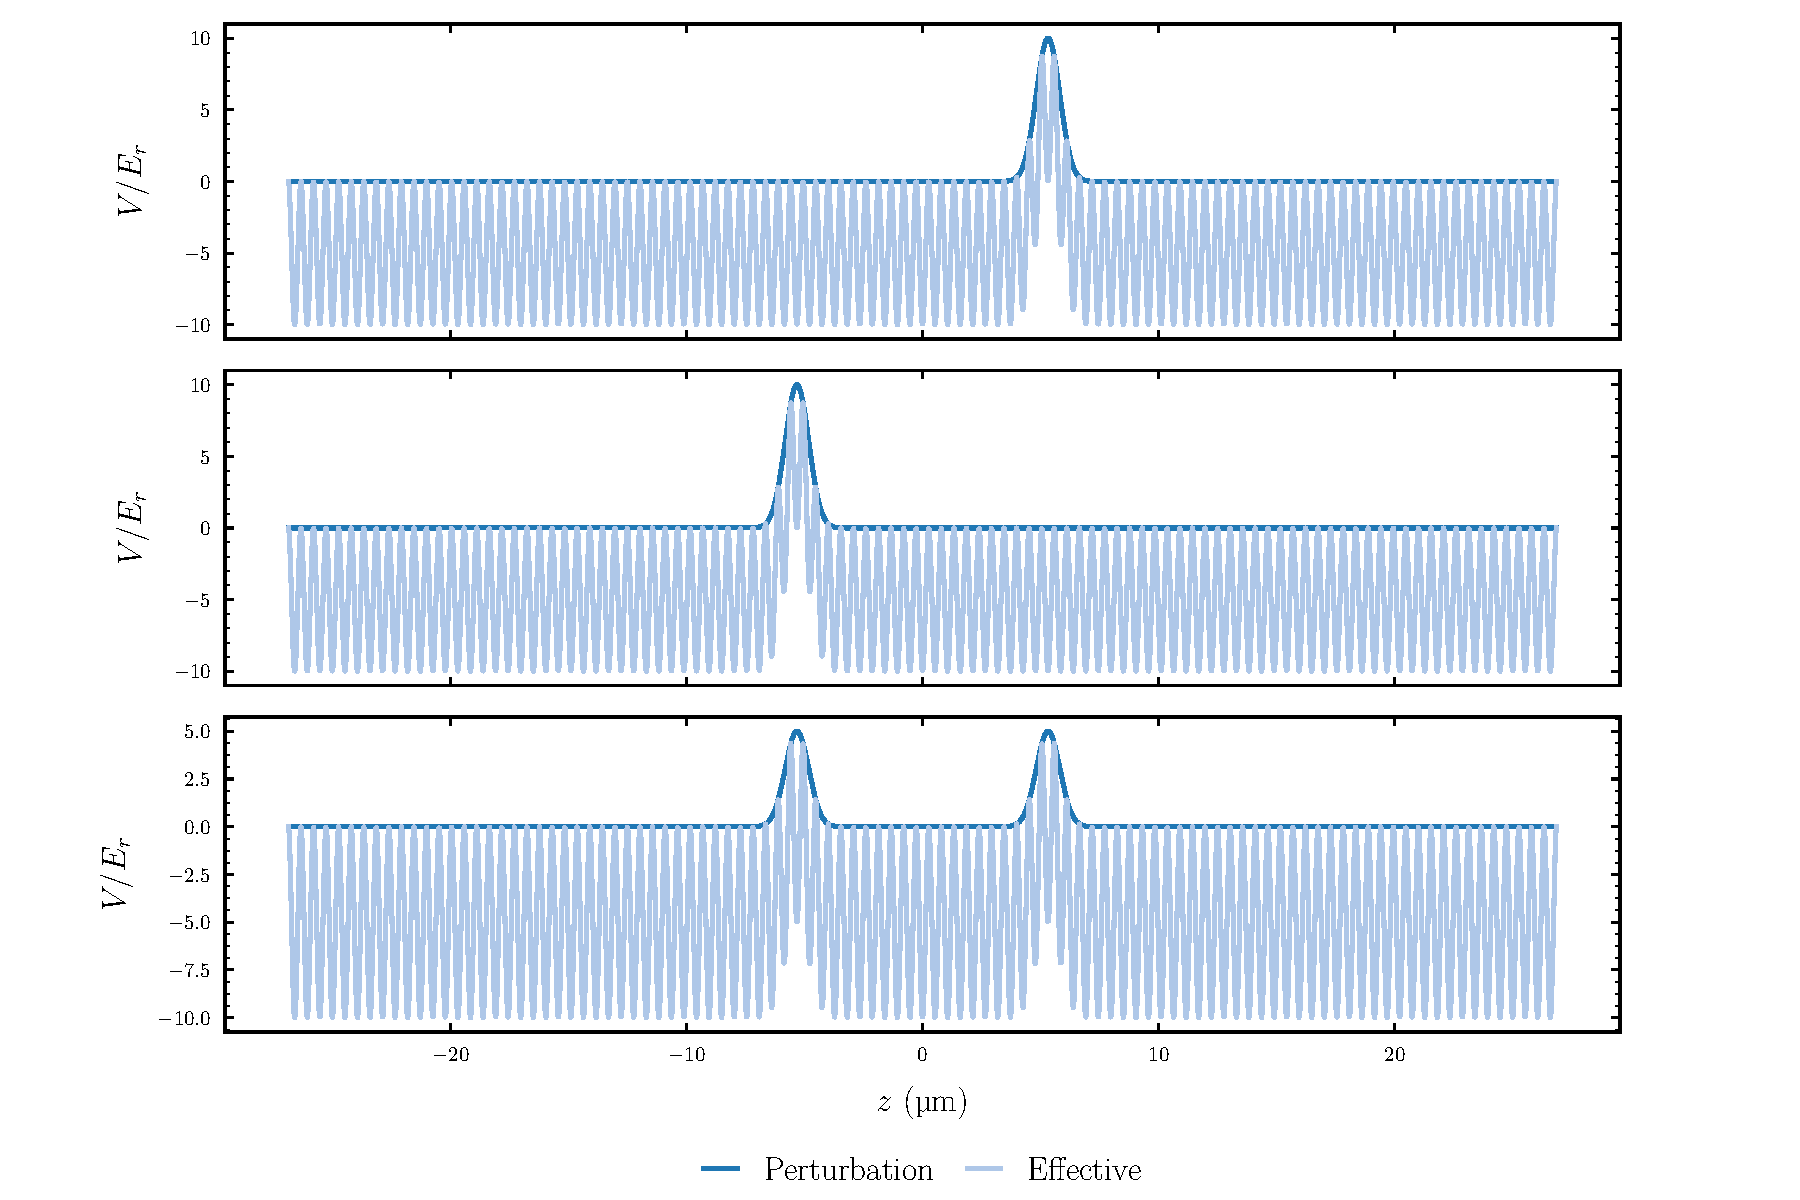
\includegraphics[width=\textwidth]{\figuredir{potential/barrier.pdf}}
  \captionsetup{width=.9\textwidth}
  \caption{Local barrier potential and lattice potential in recoil energies.
    The barrier potential is created by targetting two different focus points
    with the perturbation beam (first two rows). If both focus points are
    targetted in a sufficiently short period an average potential (last row)
    can be created.}\label{fig:effective_potential_barrier}
\end{figure}
In \Cref{fig:effective_potential_barrier} the potential energies in terms
of recoil energy are drawn for the barrier potential. To create a two sided
barrier the perturbation beam needs to change between two focus points (first
and second row). If we average over these two focus points we yield the
effective potential (third row).

\subsubsection{Pot}

As a second example of local potentials we named a pot potential that could
draw surrounding atoms.
\begin{figure}[ht]
  \centering
  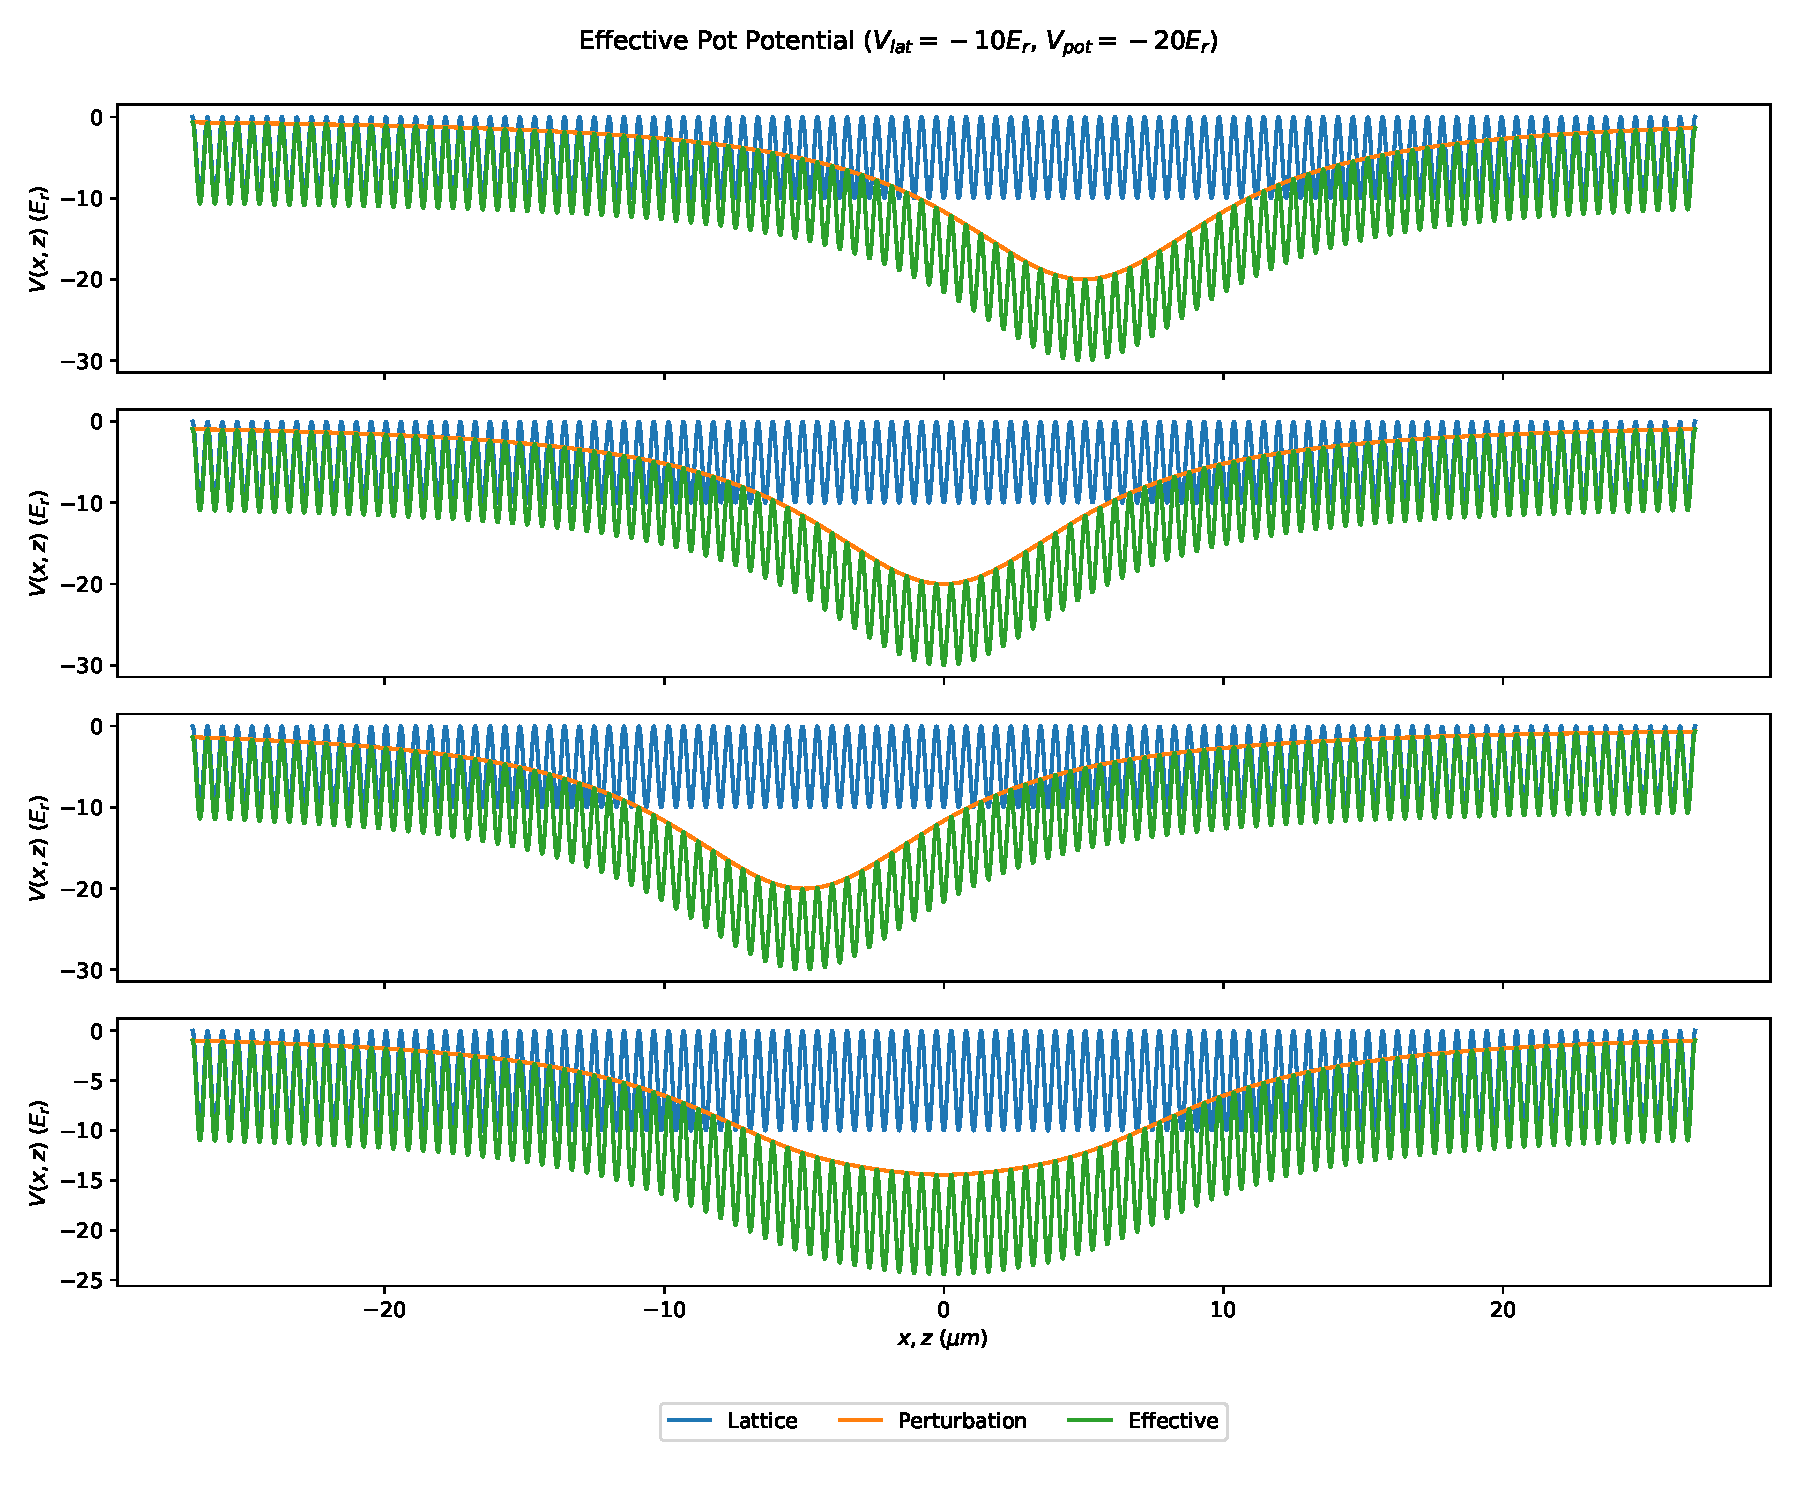
\includegraphics[width=\textwidth]{\figuredir{potential/pot.pdf}}
  \captionsetup{width=.9\textwidth}
  \caption{Local pot potential and lattice potential in recoil energies. The
    pot potential is created by targetting multiple focus points close to
  each other. Over average this yields a kind of potential
valley.}\label{fig:effective_potential_pot}
\end{figure}
\Cref{fig:effective_potential_pot} visualized such a potential. In comparison
to the barrier potential more focus points with closer distance are required.
If the focus points change in a sufficient short period an average potential
is felt by the atoms (last row) that resembles a valley.
